\section{Realization of \hp-adaptation}
\label{sec:adaptation}

For \hp{}-adaptive methods, we need to find ways to prescribe which cells are subject to which kind of adaptation. This grants awareness on how the mesh will change if adaptation is executed.

To indicate that adaptation is about to happen, we introduce general flags for refinement and coarsening into our implementation, respectively. Furthermore, to indicate that \p-adaptation is going to happen, we specify so called \textit{future finite element indices} that determine the reference finite element from the collection that will be associated to that particular cell after adaptation has been performed. They act as a counterpart to the previously introduced \textit{active finite element indices} in Sec.~\ref{sec:prerequisites}. In total, we thus have three different indicators for adaptation: Flags for refinement and coarsening, as well as future finite element indices.

To determine the extent to which cells change during the adaptation process, the affected cell properties have to be hierarchically ordered. While for \h-adaptive methods, a grid hierarchy naturally evolves from the underlying tree or forest data structure, this is not necessarily the case for \p-adaptation. Here, a hierarchy needs to be provided for the collection of reference finite elements, so that we can assign superior and subordinate elements in case of \p-refinement or \p-coarsening, respectively. For example, we arrange Lagrangian finite elements by their polynomial degree in ascending order with the largest degree on the highest level.

Executing \h-adaptation on a \p-adapted mesh reveals another challenge. We need to find a suitable finite element on cells that will be \h-adapted. During \h-refinement, we can easily choose the finite element from the parent cell for all of its children, but for \p-coarsening, the choice is not trivial. From all cells that are going to be \h-coarsened, we pick the one finite element for the parent cell from those assigned to its children that encapsulates all of them. With simultaneous \h- and \p-adaptation, future finite elements will be considered instead of the active ones. This conforms to the finite element domination logic that has been introduced by \textcite{bangerth2009} and is described in Sec.~\ref{sec:prerequisites}. An example on how finite elements are distributed during \hp-adaptation is shown in Fig.~\ref{fig:adaptation}.

\begin{figure}
\begin{subfigure}{.5\textwidth}
  \centering
  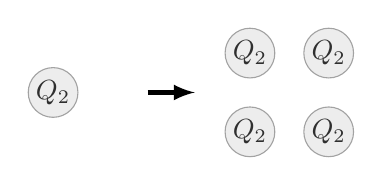
\begin{tikzpicture}[>=latex]
\def\Length{1}
\def\Radius{0.07}

% pre refinement
\LagrangeCell{0}{0}{2*\Length}{\Radius}{2}
  {{,,,,,,,,}};
\node[circle, draw=gray, fill=gray!20, inner sep=1pt, opacity=0.7, text opacity=0.8] at (\Length,\Length) {$Q_2$};

% arrow
\draw[->,ultra thick] (2.2*\Length,\Length) -- (2.8*\Length,\Length);

% post refinement
\LagrangeCell{3*\Length}{0}{\Length}{\Radius}{2}
  {{,,,,,,,,}};
\node[circle, draw=gray, fill=gray!20, inner sep=1pt, opacity=0.7, text opacity=0.8] at (3.5*\Length,0.5*\Length) {$Q_2$};

\LagrangeCell{4*\Length}{0}{\Length}{\Radius}{2}
  {{,,,,,,,,}};
\node[circle, draw=gray, fill=gray!20, inner sep=1pt, opacity=0.7, text opacity=0.8] at (4.5*\Length,0.5*\Length) {$Q_2$};

\LagrangeCell{3*\Length}{\Length}{\Length}{\Radius}{2}
  {{,,,,,,,,}};
\node[circle, draw=gray, fill=gray!20, inner sep=1pt, opacity=0.7, text opacity=0.8] at (3.5*\Length,1.5*\Length) {$Q_2$};

\LagrangeCell{4*\Length}{\Length}{\Length}{\Radius}{2}
  {{,,,,,,,,}};
\node[circle, draw=gray, fill=gray!20, inner sep=1pt, opacity=0.7, text opacity=0.8] at (4.5*\Length,1.5*\Length) {$Q_2$};
\end{tikzpicture}
  \caption{\h-refinement.}
\end{subfigure}
\begin{subfigure}{.5\textwidth}
  \centering
  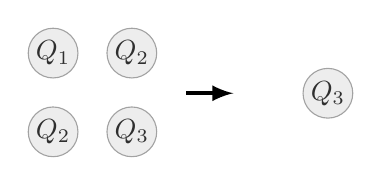
\begin{tikzpicture}[>=latex]
\def\Length{1}
\def\Radius{0.07}

% pre coarsening
\LagrangeCell{0}{0}{\Length}{\Radius}{2}
  {{,,,,,,,,}};
\node[circle, draw=gray, fill=gray!20, inner sep=1pt, opacity=0.7, text opacity=0.8] at (0.5\Length,0.5\Length) {$Q_2$};

\LagrangeCell{\Length}{0}{\Length}{\Radius}{3}
  {{,,,,,,,,,,,,,,,}};
\node[circle, draw=gray, fill=gray!20, inner sep=1pt, opacity=0.7, text opacity=0.8] at (1.5\Length,0.5\Length) {$Q_3$};

\LagrangeCell{0}{\Length}{\Length}{\Radius}{1}
  {{,,,}};
\node[circle, draw=gray, fill=gray!20, inner sep=1pt, opacity=0.7, text opacity=0.8] at (0.5\Length,1.5\Length) {$Q_1$};

\LagrangeCell{\Length}{\Length}{\Length}{\Radius}{2}
  {{,,,,,,,,}};
\node[circle, draw=gray, fill=gray!20, inner sep=1pt, opacity=0.7, text opacity=0.8] at (1.5\Length,1.5\Length) {$Q_2$};

% arrow
\draw[->,ultra thick] (2.2*\Length,\Length) -- (2.8*\Length,\Length);

% post coarsening
\LagrangeCell{3*\Length}{0}{2*\Length}{\Radius}{3}
  {{,,,,,,,,,,,,,,,}};
\node[circle, draw=gray, fill=gray!20, inner sep=1pt, opacity=0.7, text opacity=0.8] at (4*\Length,\Length) {$Q_3$};
\end{tikzpicture}
  \caption{\h-coarsening.}
\end{subfigure}
\caption[Inheritance of cell characteristics through \h-adaptation.]{Inheritance of cell characteristics through \h-adaptation in the context of \hp-adaptive meshes. With \h-refinement, all children will be associated with the parent finite element, while during \h-coarsening, the finite element space chosen on the parent cell encapsulates all those of its children ($Q_1 \subset Q_2 \subset Q_3$).}
\label{fig:adaptation}
\end{figure}

In a typical adaptation workflow, we have to distinguish between \h- and \p-adaptation. In our implementation approach, we make a complete distinction between the two at a certain point. First, corresponding cells will be either marked for refinement or coarsening and will be assigned with a corresponding general flag. On all flagged cells, we decide whether to impose \p-adaptation by setting a future finite element index or not. Now, meanings of all refinement and coarsening flags change from the general indication of adaptation to signal \h-adaptation only. If a cell shall be \p-adapted only, the corresponding flags need to be removed and only the future finite element index has to prevail, otherwise both \h- and \p-adaptation will happen simultaneously. This approach offers full flexibility to let either users decide manually how to adapt, but also provides a sufficient interface for an automatic specification of these mesh attributes, which will be described in the following section.